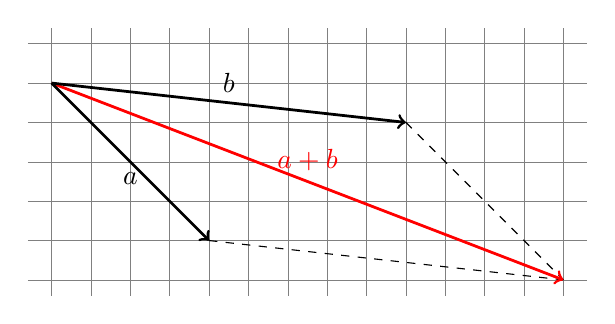
\begin{tikzpicture}[scale=1]
  \draw[step=.5cm,gray,very thin] (-2.3,-1.7) grid (4.8,1.7);
  \coordinate (A) at (-2,1);
  \coordinate (B) at (-0,-1);
  \coordinate (C) at (2.5,0.5);
  \coordinate (D) at (+2.5+2,-1+0.5-1);
  \draw[dashed] (B) -- (D);
  \draw[dashed] (C) -- (D);
  \draw[line width=1pt, red, ->] (A) -- (D) node[midway, above] {$\ve a + \ve b$};
  \draw[line width=1pt, ->] (A) -- (B) node[midway, below] {$\ve a$};
  \draw[line width=1pt, ->] (A) -- (C) node[midway, above] {$\ve b$};
\end{tikzpicture}
